\hypersetup{pageanchor=false}
\newgeometry{left=22mm,right=22mm,top=20mm,bottom=17mm}
\begin{titlepage}
\raggedright
{\large\bfseries\color{ink}УНИВЕРСИТЕТ ИТМО\par}
\vspace{3mm}{\color{accent}\rule{\textwidth}{0.7pt}\par}
\vspace{17mm}
{\large\BookAuthors\par}
\vspace{12mm}
{\fontsize{28}{34}\selectfont\bfseries\color{ink}\BookCoverTitle\par}
\vspace{8mm}
{\large Лабораторный практикум\par}
\vspace{8mm}
\noindent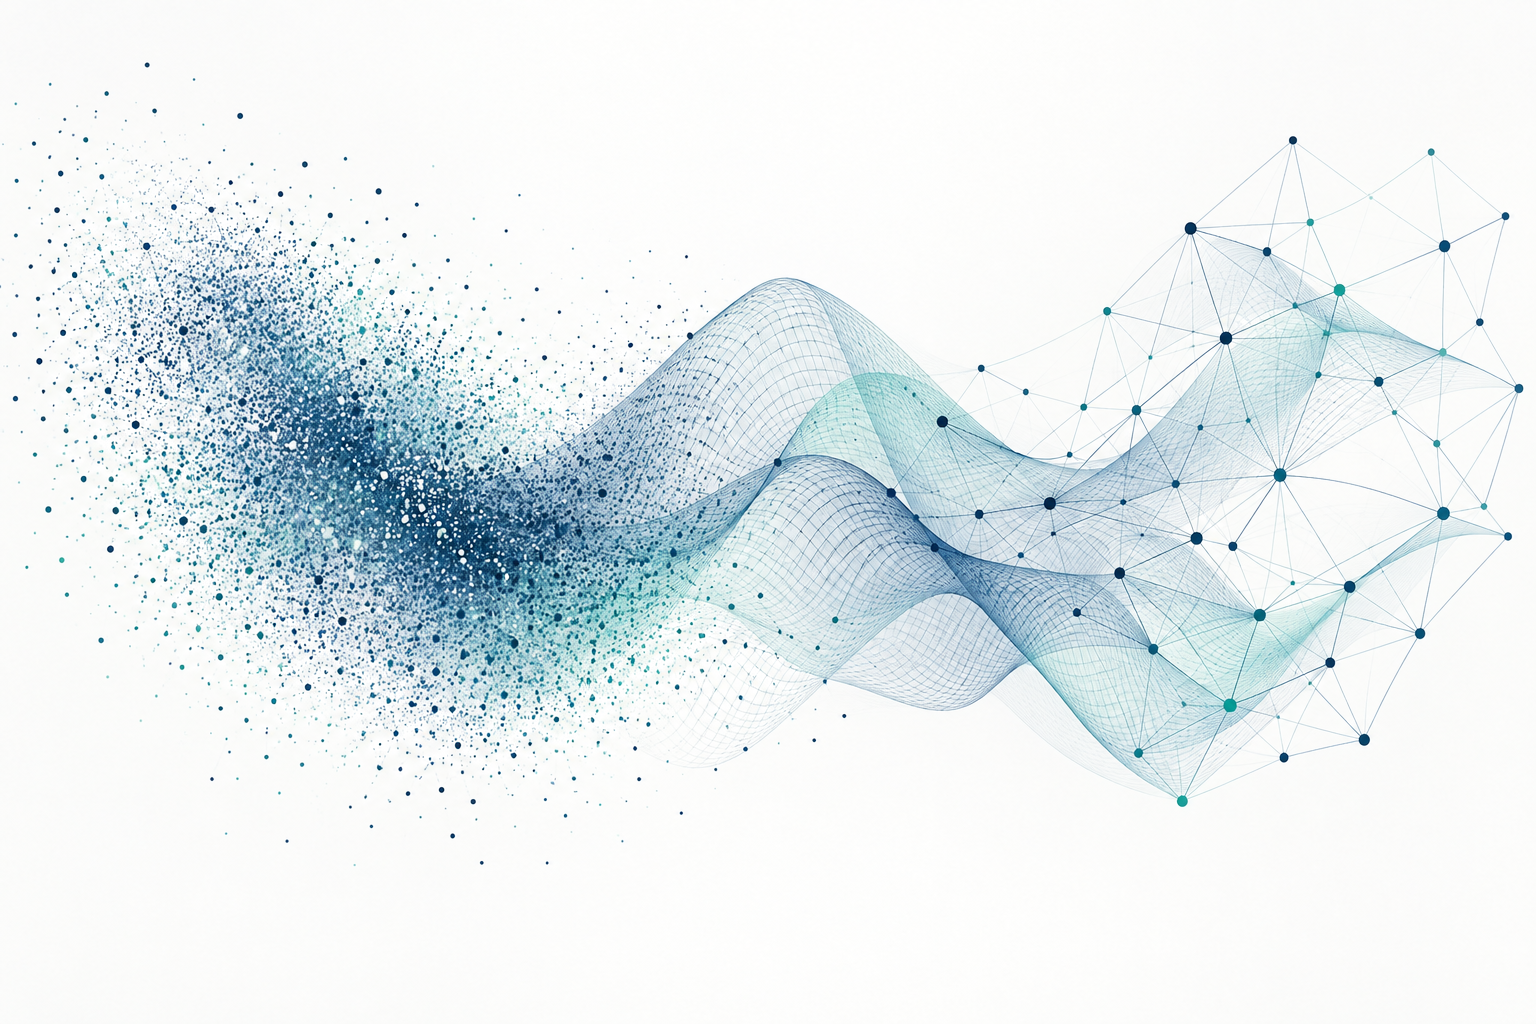
\includegraphics[width=\textwidth]{figures/cover.png}\par
\vfill
\noindent{\small\BookCity}\hfill{\small\BookYear}\par
\end{titlepage}
\restoregeometry
\setcounter{page}{1}\hypersetup{pageanchor=true}\thispagestyle{empty}
\begin{center}
{\small МИНИСТЕРСТВО НАУКИ И ВЫСШЕГО ОБРАЗОВАНИЯ\par РОССИЙСКОЙ ФЕДЕРАЦИИ\par}
\vspace{3mm}УНИВЕРСИТЕТ ИТМО\par
\vspace{23mm}{\large\BookAuthors\par}
\vspace{13mm}{\LARGE\bfseries\BookTitle\par}
\vspace{12mm}{\large ЛАБОРАТОРНЫЙ ПРАКТИКУМ\par}
\end{center}
\vfill\begin{center}\BookCity\par\BookYear\end{center}
\clearpage\thispagestyle{empty}
\begingroup\small\singlespacing
\noindent\BookAuthorsBib\ \BookTitle: лабораторный практикум. --- \BookCity: Университет ИТМО, \BookYear. --- \pageref*{LastPage}~с.
\par\bigskip
\noindent\textbf{Авторы:} \BookAuthorsFull.
\par\bigskip
\noindent\textbf{Рецензент:} \BookReviewer.
\par\bigskip
Практикум включает три работы: распознавание активности человека по признакам сигналов мобильных сенсоров; прогнозирование стоимости жилья полносвязной нейронной сетью; классификацию изображений цветов с использованием свёрточных сетей и переноса обучения. Для каждой работы приведены необходимые теоретические сведения, порядок выполнения, план исследования, контрольные точки и вопросы защиты.
\par\bigskip
Материал предназначен для студентов бакалавриата, изучающих дисциплину «Прикладной искусственный интеллект» и впервые знакомящихся с машинным обучением. Предполагаются навыки Python, работы с массивами и таблицами, знакомство со средним и производной. Основные понятия машинного обучения вводятся в самом практикуме. Сопровождающий комплект содержит учебные ноутбуки и код. Основные инструменты: scikit-learn, TensorFlow/Keras и PyTorch.
\par\bigskip
Особое внимание уделено корректному разделению данных, сопоставимости экспериментов, анализу ошибок и воспроизводимости результатов. Численные результаты опытов студент получает самостоятельно; в тексте приведены явно обозначенные расчётные примеры.
\par\bigskip
\noindent\textbf{Об Университете ИТМО}
\par\medskip
Университет ИТМО --- национальный исследовательский университет в Санкт-Петербурге. Его научные и образовательные направления включают информационные технологии и искусственный интеллект, фотонику, робототехнику, квантовые коммуникации, науки о жизни, искусство и научную коммуникацию. ИТМО участвует в программе «Приоритет-2030», развивает междисциплинарные исследования и индивидуальные образовательные траектории. С 2019 года университет самостоятельно присуждает учёные степени кандидата и доктора наук.
\par\bigskip
\noindent\copyright~Университет ИТМО, \BookYear\par
\noindent\copyright~Ким С.\,А., Евстафьев О.\,А., \BookYear
\endgroup
